\documentclass{article}
\usepackage[utf8]{inputenc}

\title{Linear Regression}
\date{}

\usepackage{amsmath}
\usepackage{amssymb}
\usepackage{natbib}
\usepackage{graphicx}

\begin{document}

\section{Fitting}
One of the central goals of machine learning is to make predictions about the future using data you have collected from the past. Machine learning is particularly effective when you have large amounts of data that allow the machine to automatically learn the patterns of interest from the data itself.

For example, say we are thinking about selling our house and we want to predict how much it will sell for based on the information about the house (e.g., how big it is, how many bathrooms, if there is a garage, etc.). Instead of trying to write out a program to determine the price by hand, we will give historical data to the computer and let it learn the pattern.

The most crucial thing in machine learning is the data you give it to learn from. A popular saying amongst machine learning practitioners goes "Garbage in, Garbage out". So before we actually talk about how to make a machine learn, we need to talk about data and the assumptions we will make about the world.

Sticking with the housing example our goal will be to predict how much our house will sell for by using data from previous house-sales in neighborhoods similar to mine. We'll suppose we have a dataset with this information that has examples of $n$ houses and what they sold for.

\begin{align*}
    (x_1, y_1) &= (2318\ \text{sq.ft.}, \$315\text{k})\\
    (x_2, y_2) &= (1985\ \text{sq.ft.}, \$295\text{k})\\
    (x_3, y_3) &= (2861\ \text{sq.ft.}, \$370\text{k})\\
    \ &\vdots \\
    (x_n, y_n) &= (2055\ \text{sq.ft.}, \$320\text{k})\\
\end{align*}

 The way we represent our data is a $n$ input/output pairs where we use the variable $x$ to represent the input and $y$ to be the output. Each example in our dataset will have \textbf{input data}, represented with the variable $x$. In our context of housing prices, there is one data input for each house (the square footage), but in other contexts, we will see that we are allowed to have multiple data inputs. The \textbf{outcome} for the house is its sale price, and we use the variable $y$ to represent that. Do note that this $y$ variable generally goes by many names such as \textbf{outcome/response/target/label/dependent variable}.
 
\textit{Notation:} We use the notation $y \in \mathbb{R}$ to say that $y$ is a real number (e.g, 14.8359) as a way to specify formally what types of values the outcome can take. Similarly, we use the notation $x \in \mathbb{R}^d$ to say that $x$ is a $d$-dimensional vector, where each entry is a real number for the $d$ data-inputs. If you aren't super familiar with vectors, that's okay, we need a deep understanding of them in this course other than they are like arrays or lists of numbers. A $d$-dimensional vector is like a list of numbers of length $d$. In our example of housing, we would write $x \in \mathbb{R}^1$ which is the same as $x \in \mathbb{R}$ since there is only 1 data input.

We are going to make an assumption that there is a relationship between the square footage of the house and its sale price. We are going to say that there exists some secret (unknown) function $f$ such that the price of a house is approximately equal to the function's output for the houses input data. With notation, we write this:
$$y \approx f(x)$$

We are not saying that the output has to be exactly equal, but rather that it is close. The reason we allow for this wiggle-room is that we are allowing for the fact that our model of the world might be slightly wrong. There are probably more factors outside the square footage that affect a house's price, so we won't find an exact relationship between this input and our output. Another reason to allow this approximation for our model is to allow for the fact that measuring the square footage of a house, might not be an exact science.

To be a bit more precise about how we believe the world works, we will use a very common assumption about how we think the world will work. We first show the formula, and then explain the parts.

$$y_i = f(x_i) + \epsilon_i$$

\textit{Notation:} When we subscript a variable like $x$ to be $x_i$, it means we are talking about the $i^{th}$ example from our dataset. When we use $x$ without subscripts, we are talking about a generic house, while when I say $x_{12}$, I am talking about the $12^{th}$ house in the dataset we were given.

The way to read this formula above is to say that the outcomes we saw, $y_i$, come from the true function $f$ being applied to the input data $x_i$, but that there was some noise $\epsilon_i$ added to it that may cause some error. The animation below shows a visual representation of this model. This is a challenge that our machine learning model will need to overcome: we don't have access to the true function and have to try to learn it (so we can make predictions about new houses) while only having these noisy approximations.

TODO Animation

\begin{figure}[h!]
\centering
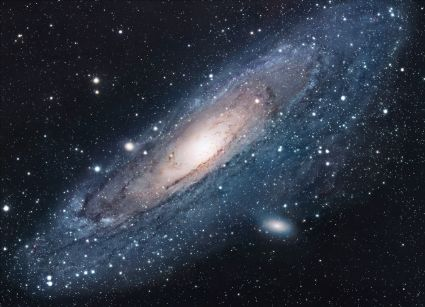
\includegraphics[scale=1.7]{universe}
\caption{The Universe}
\label{fig:universe}
\end{figure}

\section{Conclusion}
``I always thought something was fundamentally wrong with the universe'' \citep{adams1995hitchhiker}

\bibliographystyle{plain}
\bibliography{references}
\end{document}
